\section{Evaluation}

To demonstrate the performance and correctness of our ZOne implementation, we
present three benchmark: convolution, Black-Scholes, European pricing, and histogram.
While all three benefit greatly from our I/O latency interleaving, we show
  that histogram also improves from our compiler optimizations.


\subsection{Convolution}

\begin{figure}
\centering
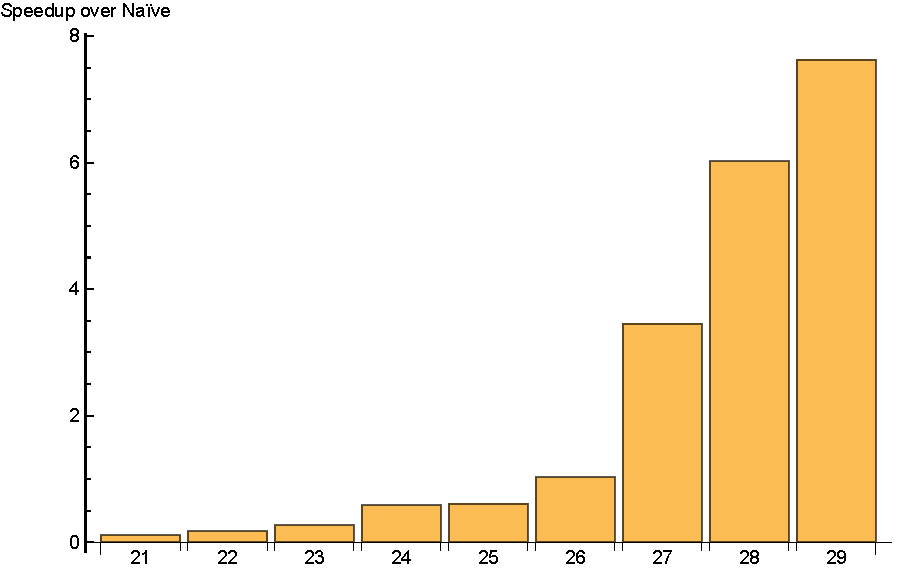
\includegraphics[scale=0.5]{data/stencil.pdf}
\caption{Speedup of convolution over naive CUDA implementation.
  The $x$-axis is the convolved vector size in bytes.}
\label{fig:stencil}
\centering
\end{figure}

Convolutions has wide applications in both engineering and mathematics.
Depending on the ``kernel'' (or mask), convolution, or stencil as it is sometimes called,   can be used to approximate a differential operator ---
 a $[-\frac{1}{h}, 0, \frac{1}{h}]$ kernel approximates the gradient operator, for example.
High-performance CPU convolution implementations
involve vectorization and tiling to make full use of cache bandwidth and
execution resources.
The biggest impact from a GPU point of view, however, is the use of fast
  scratch pad memory as a user managed cache.
We therefore see little performance benefits from our compiler passes, and the
  performance primarily stems from interleaving memory copies.
Figure~\ref{fig:stencil} shows the speedup achieved by our runtime for a 1D
  convolution compared to a naive CUDA implementation.


\subsection{Option Pricing}

\subsubsection{Black-Scholes}
Black-Scholes models option pricing by simplifying its formula, and some other stuff....


Coarsening increases register pressure, and degrades performance.


\begin{figure}
\centering
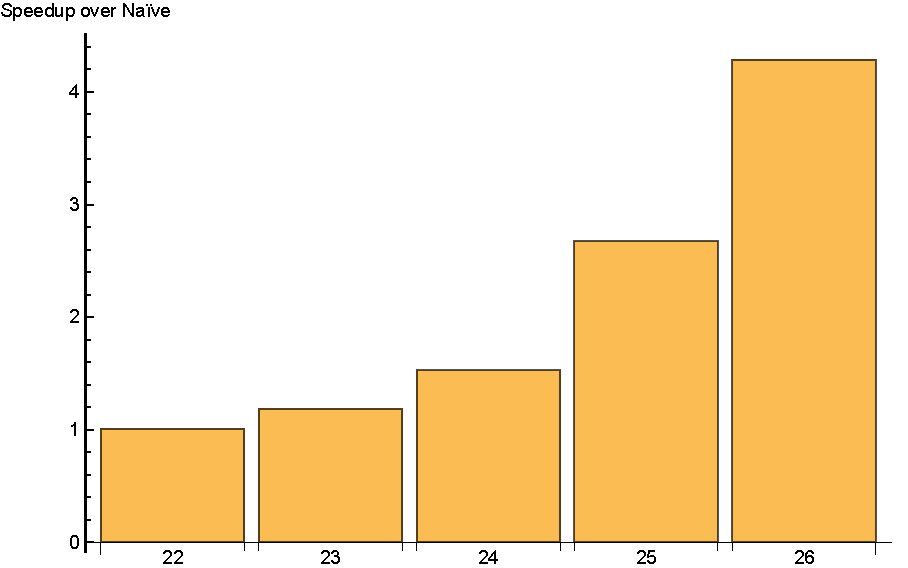
\includegraphics[scale=0.5]{data/blackscholes.pdf}
\caption{Speedup over CUDA version..todo}
\label{fig:blackscholes}
\centering
\end{figure}


\subsubsection{European Options}

\subsection{Binary Image Segmentation}

\begin{figure}
\centering
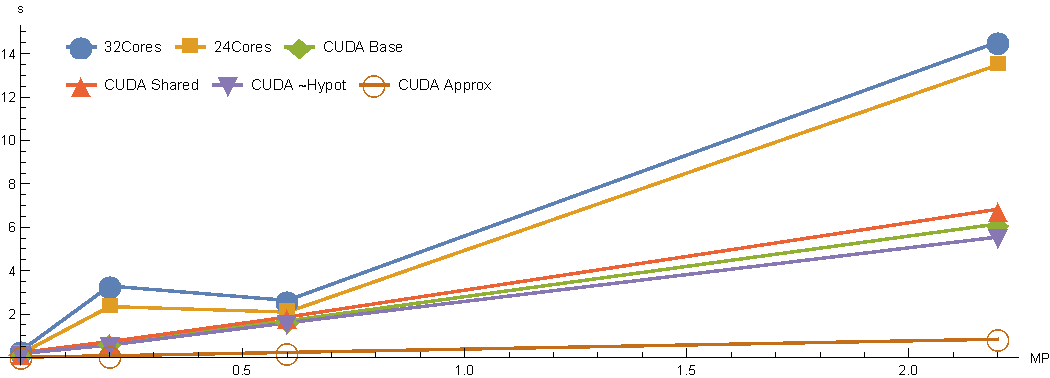
\includegraphics[scale=0.4]{fig/growcut.pdf}
\caption{This shows the timing of GrowCut on a $24$ and $32$ core system.
As expected, no difference is noticed between the two configurations due to hitting I/O
bandwidth limits. The $x$ axis is the number of megapixels in the image and the $y$ axis is the execution time in seconds.}
\label{fig:growcut}
\centering
\end{figure}

Binary image segmentation partitions an image into foreground and background
  pixels.
GrowCut~\cite{vezhnevets2005growcut} is an algorithm that uses ideas from cellular automaton to perform image
  sgementation.
GrowCut flood
  neighbors based on an initial seed until it reaches a barrier.
One can think of each pixel as a bacteria with an energy function, if a bacteria has
  higher energy than one of its neighbors, then it will devour them --- otherwise it
  is the victim.
The algorithm is iterated until either a fixed point is reached or the maximum number
  of iterations are reached.
A pseudocode of the algorithm is shown bellow:


\begin{lstlisting}
Input: Image, Approximate Label
Output: Label Sgementation
-----------------------------
changed = true
do_wile changed || iterations < MAX_ITERATIONS:
  changed = false
  for ii from 0 to height:
    for jj from 0 to width:
      cp = image[ii][jj]
      nl = lp = label[ii][jj]
      ns = sp = strength[ii][jj]
      for ni from -1 to 1:
        for nj from -1 to 1:
          cq = image[ii+ni][jj+nj]
          lq = label[ii+ni][jj+nj]
          sq = strength[ii+ni][jj+nj]
          gc = g(cp, cq)
          if gc * sq > sp:
            nl = lq
            ns = sq * gc
            changed = true
          end
        end
      end
      nextLabel[ii][jj] = nl
      nextStrength[ii][jj] = ns
    end
  end
  label = nextLabel
  strength = nextStrength
end
\end{lstlisting}

For our experiments, we set \fix{MAX\_ITERATIONS} to $2048$ and use a
  simple penatly function $g(x,y)  = 1 - \frac{\|x - y\|}{255}$.

We use this algorithm to show that a platau is reached in terms of scaling.
Using a standard sgementation dataset~\cite{gridcut}, we modified our runtime so
  it does not use the GPU and use TBB for threading. figure~\ref{fig:growcut} shows the
  performance on a multicore machine as well as on a GPU as the input
  size varies.
We see that having $24$ vs $32$ cores does not make a difference for streaming, since
  one hits the I/O bandwidth limits.
More advanced I/O configurations, such as RAID, would allow us to scale better as the number of cores become large. 

\subsection{Histogram}

\begin{figure}
\centering
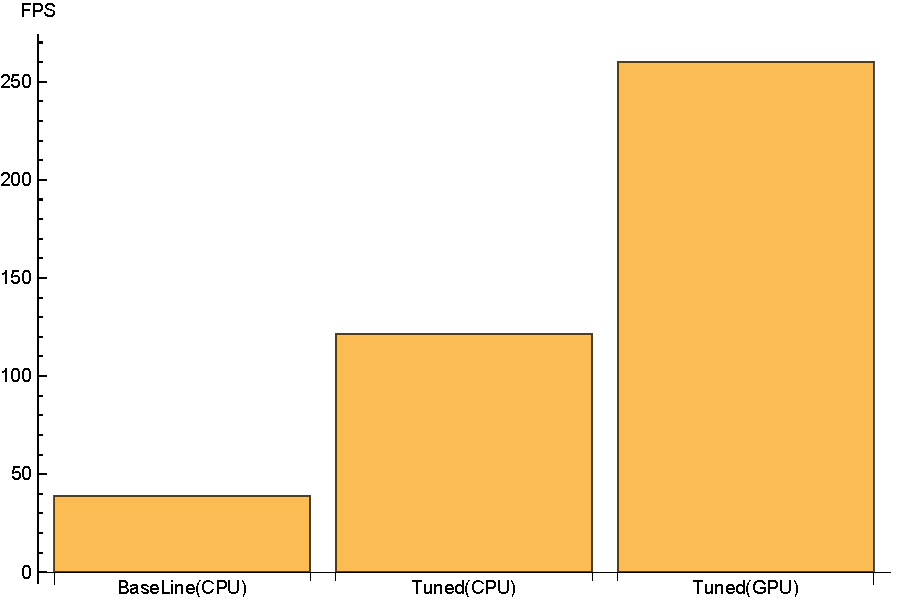
\includegraphics[scale=0.5]{data/histogram.pdf}
\caption{Frames per seconds achieved for histogram equalization kernel on a 4K video. The figure compares the tuned GPU implementation to a naive CPU and tuned CPU implementations. The tuned GPU implementation uses thread coarsening to achieve high fps.}
\label{fig:histogram}
\centering
\end{figure}


\begin{figure}
\centering
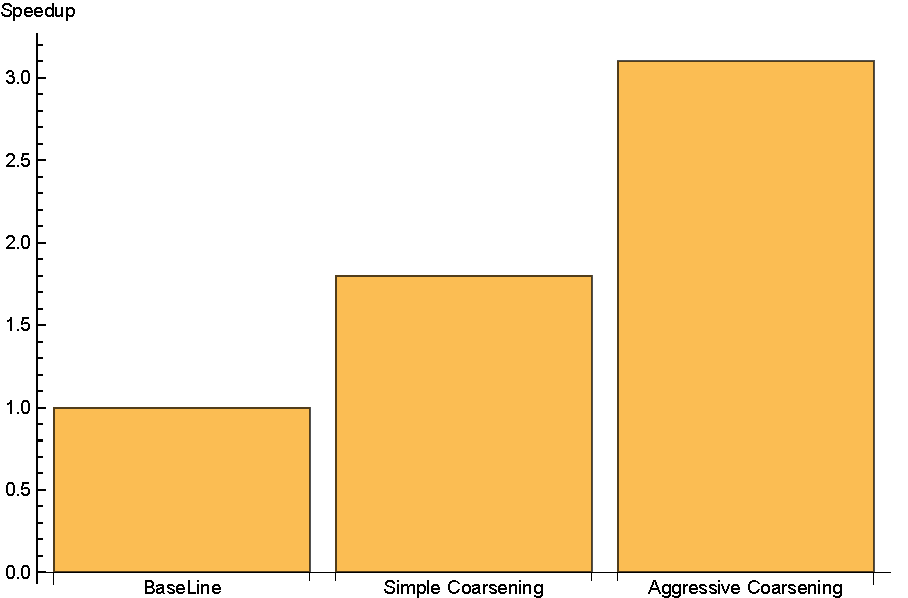
\includegraphics[scale=0.5]{data/histogramc.pdf}
\caption{The coarsening parameter impacts the performance of the histogram equalization kernel.}
\label{fig:histogramCoarsining}
\centering
\end{figure}

Histograms are a fundamental analysis tool in image and data processing.
Although serial  histogram implementations are very straightforward, efficient parallel histogram implementations are
more involved due to the data-dependent access pattern. 
Atomic memory operations are typically used to enable potential parallelism for data-dependent stores. 
Privatization, where individual histograms for portions of the data are computed separately
and then compiled together into the overall result, may potentially reduce memory contention and then penalty of serialization.
Also, scan or sort operations on input data can potentially replace atomic memory operations, and achieve the similar functionality.

In this image histogram equalization benchmark, atomic memory operations are specifically applied. 
Figure \ref{fig:histogram} shows the performance difference among serial CPU, efficient parallel CPU, and efficient parallel GPU versions of image histogram equalization on a 4K video.
Our GPU image histogram equalization can achieve up to 260.2 fps on a Tesla C2050, while serial and parallel CPU versions only have 39.1 and 120.5 fps, respectively, on a Intel Xeon E5520 CPU.
Tiling and thread coarsening are the two major optimization involved in this evaulation.
In the histogram kernel particularly, tiling (baseline in Figure \ref{fig:histogramCoarsining}) is simply applied for further optimization in order to gain memory efficiency.
Beyond tiling, thread coarsening (simple coarsening in Figure \ref{fig:histogramCoarsining}) can be applied for hiding the overhead of kernels and give a 1.78x speedup over the tiling version.
An aggressive thread coarsening version (aggressive coarsening in Figure \ref{fig:histogramCoarsining}), which involves loop fusion of independent histograms, can further have up to 3.10x over the tiling version.


